\documentclass[sigconf, anonymous]{acmart}

\fancyhf{} % Remove fancy page headers
\fancyhead[C]{Anonymous submission \#9999 to ACM CCS 2019} % TODO: replace 9999 with your paper number
\fancyfoot[C]{\thepage}

\setcopyright{none} % No copyright notice required for submissions
\acmConference[Anonymous Submission to ACM CCS 2019]{ACM Conference on Computer and Communications Security}{Due 15 May 2019}{London, TBD}
\acmYear{2019}

\settopmatter{printacmref=false, printccs=true, printfolios=true} % We want page numbers on submissions

%%\ccsPaper{9999} % TODO: replace with your paper number once obtained

\begin{document}
\title{A Gas-Efficient Superlight \\Bitcoin Client in Solidity}

\begin{abstract}

Superlight clients enable the verification of proof-of-work-based blockchains
by checking only a small representative number of block headers instead of all
the block headers as done in SPV. Such clients can be embedded within other
blockchains by implementing them as smart contracts, allowing for cross-chain
verification. One such interesting instance is the consumption of Bitcoin data
within Ethereum by implementing a Bitcoin superlight client in Solidity. While
such theoretical constructions have demonstrated security and efficiency, no
practical implementation exists. In this work, we put forth the first practical
Solidity implementation of a superlight client which implements the NIPoPoW
superblocks protocol. Contrary to previous work, our Solidity smart contract
achieves sufficient gas-efficiency to allow a proof and counter-proof to fit
within the gas limit of a block, making it practical. We provide extensive
experimental measurements for gas. The optimizations that enable gas-efficiency
heavily leverage a novel technique which we term hash-and-resubmit, which
almost completely eliminates persistent storage requirements, the most
expensive operation of smart contracts in terms of gas. Instead, the contract
asks contesters to resubmit data and checks their veracity by hashing it. We
show that such techniques can be used to bring down gas costs significantly and
may have applications to other contracts. We also identify and rectify multiple
implementation security issues of previous work such as premining
vulnerabilities. Lastly, our implementation allows us to calculate concrete
cryptoeconomic parameters for the superblocks NIPoPoWs protocol and in
particular to make recommendations about the monetary value of the collateral
parameters. We provide such parameter recommendations over a variety of
liveness and adversarial bound settings.

\end{abstract}

% TODO: replace this section with code generated by the tool at
% https://dl.acm.org/ccs.cfm

\begin{CCSXML}
<ccs2012>
<concept>
<concept_id>10002978.10003029.10011703</concept_id>
<concept_desc>Security and privacy~Usability in security and privacy</concept_desc>
<concept_significance>500</concept_significance>
</concept>
</ccs2012>
\end{CCSXML}

\ccsdesc{Security and privacy~Use https://dl.acm.org/ccs.cfm to generate actual concepts section for your paper}
% -- end of section to replace with generated code

\keywords{template; formatting; pickling} % TODO: replace with your keywords

\maketitle

\section{Introduction}

Blockchain interoperability~\cite{dionyziz} is the ability of distinct
blockchains to communicate.  This \emph{crosschain}~\cite{pow-sidechains,
pos-sidechains,burn,crosschain-sok, gtklocker} communication enables useful
features across blockchains such as the transfer of assets from one chain to
another (one-way peg) and back (two-way peg)~\cite{pow-sidechains}. To date,
there is no commonly accepted decentralized protocol that enables cross-chain
transactions. Currently, crosschain operations are only available to the users
via third-party applications, such as multi-currency wallets. However, this
treatment is opposed to the nature of decentralized currencies.

\noindent

In general, crosschain-enabled blockchains A, B support the following
operations:

\begin{itemize}
\item Crosschain trading: a user with deposits in blockchain A, makes a
    payment to a user in blockchain B.
\item Crosschain fund transfer: a user transfers her funds from blockchain
    A to blockchain B. After the transfer, these funds no longer exist in
    blockchain A. The user can later decide to transfer any portion of the
    original amount to the blockchain of origin.
\end{itemize}


\noindent

In order to perform crosschain operations, there must be a mechanism that
allows users of blockchain A to discover events that have occurred in chain B,
such as transactions. A trivial manner to perform such an audit is to
participate as a full node in multiple chains. This approach, however, is
impractical because a sizable amount of storage is needed to host entire
chains as they grow in time. As of June 2020, Bitcoin~\cite{nakamoto} chain
spans roughly 245 GB, and Ethereum~\cite{wood, buterin} has exceeded 300
GB\footnote{Size of blockchain derived from https://www.statista.com,
https://etherscan.io}. Naturally, not all users are
able to accommodate this size of data, especially if portable devices are used,
such as mobile phones.

One early solution to compress the extensive size of blockchain is addressed by
Nakamoto~\cite{nakamoto} with the Simplified Payment Verification (SPV)
protocol. In SPV, only the headers of blocks are stored, saving a considerable
amount of storage.  However, even with this protocol, the process of
downloading and validating all block headers still demands a considerable
amount of resources since they grow linearly to the size of the blockchain.
In Ethereum, for instance, headers sum up to approximately 4.8
GB\footnote{Calculated as the number of blocks (10,050,219) times the size of
header (508 bytes). Statistics by https://etherscan.io/} of data. A mobile
client needs several minutes, even hours, to fetch all information needed in
order to function as an SPV client.

Towards the goal of delivering more practical solutions for blockchain
transaction verification, a new generation of \emph{superlight}
clients~\cite{popow, nipopows, compactsuperblocks, flyclient} emerged. In these
protocols, cryptographic proofs are generated, that prove the occurrence of
events inside a blockchain. These proofs require only a polylogarithmic size of
data compared to the SPV model, resulting into better performance. By utilizing
superlight client protocols, a compressed proof for an event in chain A is
constructed and dispatched to chain B. If chain B supports smart contracts, the
proof is then verified automatically and transparently \emph{on-chain}. This
communication is realized without the intervention of third-party applications.
An interesting application of such a protocol is the communication between
Bitcoin and Ethereum.

\noindent

\textbf{Related Work.} We use Non-Interactive Proofs of Proof of Work
(NIPoPoWs)~\cite{nipopows, pow-sidechains} as the fundamental building block of
our solution. This cryptographic primitive is \emph{provably secure} and
provides \emph{succinct proofs} regarding the existence of an arbitrary event
in a chain. Contrary to the linear growth rate of the underlying blockchain,
NIPoPoWs span polylogarithmic size of blocks. A few cryptocurrencies already
include built-in NIPoPoWs support. ERGO~\cite{ergo}, Nimiq~\cite{nimiq}, and
WebDollar~\cite{webdollar} have added support since their genesis.

Christoglou~\cite{gglou} provided a Solidity smart contract which is the first
implementation of crosschain events verification based on NIPoPoWs, where
proofs are submitted and checked for their validity. This solution, however, is
impractical due to extensive usage of resources, widely exceeding the Ethereum
block gas limit.

Other attempts have been done to address the verification of Bitcoin
transactions to the Ethereum blockchain, most notably BTC
Relay~\cite{btcrelay}.

\noindent

\textbf{Our contribution.} Notably, no practical implementation for superlight
clients exists to date. In this paper, we focus on constructing a practical
client for NIPoPoWs. For the implementation of our client, we refine the
NIPoPoW protocol based on a series of keen observations. These refinements
allow us to leverage useful techniques that construct a practical solution for
proof verification. We believe that this achievement is a decisive step towards
the establishment of NIPoPoWs to the application end, therefore it is a
significant progress in order to provide a widely accepted protocol that
enables crosschain transactions. A summary of our contributions in this paper
is as follows:
\begin{enumerate}
\item We developed the first decentralized client that securely verifies
crosschain events and is practical. Our client establishes a trustless and
efficient solution to the interoperability problem. We implement\footnote{Our
implementation, unit tests and experiments can be found in https://github.com/superlightBitcoinClientInSolidity/verifier} our client
in Solidity, and we verify Bitcoin events to the Ethereum blockchain. The
security assumptions we make are no other than
SPV's~\cite{eclipse, eclipse-ethereum}.
\item We present a novel pattern which we term \emph{hash-and-resubmit}. Our
pattern significantly improves performance of Ethereum smart
contracts~\cite{wood, buterin} in terms of gas consumption by utilizing the
\emph{calldata} space of Ethereum blockchain to eliminate high-cost storage
operations.
\item We create an \emph{optimistic} schema which we incorporate into the design
of our client. This design achieves significant performance improvement by
replacing linear complexity verification of proofs, with constant complexity
verification.
\item We demonstrate via application that the NIPoPoW protocol is practical,
making the cryptographic primitive the first provably secure construction of
succinct proofs that is efficient to implement.
\item We present an econometric analysis on NIPoPoWs. This analysis allows us
to provide concrete values of collateral parameters in fiat, as well as the
cost of submit and contest actions under different gas price configurations.

\end{enumerate}

Our implementation meets the following requirements:
\begin{enumerate}
\item Security: The client implements a provably secure protocol.
\item Decentralization: The client is not dependent on third-party applications
and operates in a transparent, decentralized manner.
\item Efficiency: The client comply with all environmental constraints, i.e.\
block gas limit and calldata size limit of the Ethereum blockchain.
\end{enumerate}

We selected Bitcoin as the source blockchain as it the most used cryptocurrency,
and enabling crosschain transactions in Bitcoin is beneficial to the vast
majority of the blockchain community. We selected Ethereum as the target blockchain
because, besides its popularity, it supports smart contracts, which is a
requirement in order to perform on-chain verification.

% Bitcoin does not include interlink structures in blocks. The setting we refer
% to is a hard fork~\cite{hard-fork}, but we believe that a
% velvet~\cite{velvet-fork} fork can also be supported as it does not add
% significant overhead to the verifier as shown in ~\cite{andri}.

\noindent
\textbf{Structure.} In Section 2 we describe the blockchain technologies that
are relevant to our work. In Section 3 we put forth the
\emph{hash-and-resubmit} pattern. We demonstrate the improved performance of
smart contracts using the pattern, and how it is incorporated into our
client. In Section 4, we present an alteration of the NIPoPoW protocol that
enables the elimination of look-up structures. This allows for efficient
interactions due to the considerably smaller size of dispatched proofs. In
Section 5, we put forth an optimistic schema that significantly lowers the
complexity of a proof's structural verification from linear to constant, by
introducing a new interaction which we term \emph{dispute phase}. Furthermore,
we present a technique that leverages the dispatch of a constant number of blocks
in the contest phase. Finally, in Section 6, we present our cryptoeconomic analysis
on our client. We establish the monetary value of collateral parameters, as well
as the cost of each interaction with the client for different gas prices.

% \section{Preliminaries}\label{sec:preliminaries}

\noindent
\textbf{Model.}
We consider a setting where the blockchain network consists of two different
types of nodes: The first kind, \emph{full nodes}, are responsible for the
maintenance of the chain including verifying it and mining new blocks. The
second kind, \emph{verifiers} connect to full nodes and wish to learn facts
about the blockchain without downloading it, for example whether a particular
transaction is confirmed. The full nodes therefore also function as
\emph{provers} for the verifiers. Each verifier connects to multiple provers, at
least one of which is assumed to be honest.

We model full nodes according to the Backbone model~\cite{backbone}. There are
$n$ full nodes, of which $t$ are adversarial and $n - t$ are honest. All $t$
adversarial parties are controlled by one colluding adversary $\mathcal{A}$. The
parties have access to a hash function $H$ which is modelled as a common Random
Oracle~\cite{ro}. To each novel query, the random oracle outputs $\kappa$ bits
of fresh randomness. Time is split into distinct \emph{rounds} numbered by the
integers $1, 2, \cdots$. Our treatment is in the \emph{synchronous model}, so we
assume messages \emph{diffused} (broadcast) by an honest party at the end of a
round are received by all honest parties at the beginning of the next round.
This is equivalent to a network connectivity assumption in which the round
duration is taken to be the known time needed for a message to cross the
diameter of the network. The adversary can inject messages, reorder them, sybil
attack by creating multiple messages, but not suppress messages.

\noindent
\textbf{Blockchain.} Each honest full node locally maintains a \emph{chain} $\chain$, a sequence of
blocks. In understanding that we are developing an improvement on top of SPV, we
use the term \emph{block} to mean what is typically referred to as a
\emph{block header}. Each block contains the Merkle Tree root~\cite{merkle} of
transaction data $\overline{x}$, the hash $s$ of the previous block in the chain
known as the \emph{previd}, as well as a nonce value $ctr$. As discussed in the
Introduction, the compression of application data $\overline{x}$ is orthogonal
to our goals in this paper and has been explored in independent
work~\cite{edrax} which can be composed with ours. Each block $b = s \conc
\overline{x} \conc ctr$ must satisfy the proof-of-work~\cite{pow} equation $H(b) \leq T$
where $T$ is a constant \emph{target}, a small value signifying the difficulty
of the proof-of-work problem. Our treatment is in the \emph{static difficulty}
case, so we assume that $T$ is constant throughout the execution\footnote{A
treatment of variable difficulty NIPoPoWs has been explored in the soft fork
case~\cite{dionyziz}, but we leave the treatment of velvet fork NIPoPoWs in the
variable difficulty model for future work.}. $H(B)$ is
known as the \emph{block id}.

Blockchains are finite block sequences obeying the \emph{blockchain property}:
that in every block in the chain there exists a pointer to its previous block. A
chain is \emph{anchored} if its first block is \emph{genesis}, denoted $\mathcal{G}$,
a special block known to all parties. This is the only node the verifier knows about
when it boots up. For chain addressing we use Python brackets $\chain[\cdot]$. A
zero-based positive number in a bracket indicates the indexed block in the
chain. A negative index indicates a block from the end, e.g., $\chain[-1]$ is
the tip of the blockchain. A range $\chain[i{:}j]$ is a subarray starting from
$i$ (inclusive) to j (exclusive). Given chains $\chain_1, \chain_2$ and blocks
$A, Z$ we concatenate them as $\chain_1 \chain_2$ or $\chain_1 A$ (if clarity
mandates it, we also use the symbol $\conc$ for concatenation). Here,
$\chain_2[0]$ must point to $\chain_1[-1]$ and $A$ must point to $\chain_1[-1]$.
We denote $\chain\{A{:}Z\}$ the subarray of the chain from block $A$ (inclusive) to
block $Z$ (exclusive). We can omit blocks or indices from either side of the range to
take the chain to the beginning or end respectively. As long as the blockchain
property is maintained, we freely use the set operators $\cup$, $\cap$ and
$\subseteq$ to denote operations between chains, implying that the appropriate
blocks are selected and then placed in chronological order.

During every round, every party attempts to \emph{mine} a new block on top of
its currently adopted chain. Each party is given $q$ queries to the random
oracle which it uses in attempting to mine a new block. Therefore the adversary
has $tq$ queries per round while the honest parties have $(n - t)q$ queries per
round. When an honest party discovers a new block, they extend their chain with
it and broadcast the new chain. Upon receiving a new chain $\chain'$ from the
network, an honest party compares its length $|\chain'|$ against its currently
adopted chain $\chain$ and adopts the newly received chain if it is longer. It
is assumed that the honest parties control the majority of the computational
power of the network. This \emph{honest majority assumption} states that there
is some $\delta$ such that $t < (1 -  \delta)(n - t)$. If so, the protocol
ensures consensus among the honest parties: There is a constant $k$, the
\emph{Common Prefix} parameter, such that, at any round, all the chains
belonging to honest parties share a common prefix of blocks; the chains can
deviate only up to $k$ blocks at the end of each chain~\cite{backbone}.
Concretely, if at some round $r$ two honest parties have $\chain_1$ and
$\chain_2$ respectively, then either $\chain_1[{:}-k]$ is a prefix of $\chain_2$
or vice versa.

\noindent
\textbf{Superblocks.}
Some valid blocks satisfy the proof-of-work equation better than required. If
a block $b$ satisfies $H(b) \leq 2^{-\mu} T$ for some natural number
$\mu \in \mathbb{N}$ we say that $b$ is a \emph{$\mu$-superblock} or a block
\emph{of level} $\mu$. The probability of a new valid block achieving level
$\mu$ is $2^{-\mu}$. The number of levels in the chain will be $\log|\chain|$
with high probability~\cite{popow}. Given a chain $\chain$, we denote
$\chain\upchain^\mu$ the subset of $\mu$-superblocks of $\chain$.

Non-Interactive Proofs of Proof-of-Work (NIPoPoW) protocols allow verifiers to
learn the most recent $k$ blocks of the blockchain adopted by an honest full
node without downloading the whole chain. The challenge lies in building a
verifier who can find the suffix of the longest chain between claims of both
honest and adversarial provers, while not downloading all block headers. Towards
that goal, the \emph{superblock} approach uses superblocks as samples of
proof-of-work. The prover sends superblocks to the verifier to convince them
that proof-of-work has taken place without actually presenting all this
proof-of-work. The protocol is parametrized by a constant security parameter
$m$. The parameter determines how many superblocks will be sent by the prover to
the verifier and security is proven with overwhelming probability in $m$.

\noindent
\textbf{Prover.}
The prover selects various levels $\mu$ and for each such level sends a
carefully chosen portion of its $\mu$-level \emph{superchain}
$\chain\upchain^\mu$ to the verifier. In standard blockchain protocols such as
Bitcoin and Ethereum, each block $\chain[i + 1]$ in $\chain$ points to its
previous block $\chain[i]$, but each $\mu$-superblock $\chain\upchain^\mu[i +
1]$ does not point to its previous $\mu$-superblock $\chain\upchain^\mu[i]$. It
is imperative that an adversarial prover does not reorder the blocks within a
superchain, but the verifier cannot verify this unless each $\mu$-superblock
points to its most recently preceding $\mu$-superblock. The proposal is
therefore to \emph{interlink} the chain by having each $\mu$-superblock include
an extra pointer to its most recently preceding $\mu$-superblock. To ensure
integrity, this pointer must be included in the block header and verified by
proof-of-work. However, the miner does not know which level a candidate block
will attain prior to mining it. For this purpose, each block is proposed to
include a pointer to the most recently preceding $\mu$-superblock, for every
$\mu$, as illustrated in Figure~\ref{fig.hierarchy}. As these levels are only
$\log|\chain|$, this only adds $\log|\chain|$ extra pointers to each block
header.

\begin{algorithm}
    \caption{\label{alg.nipopow-prover}The \textsf{Prove} algorithm
    for the NIPoPoW protocol in a soft fork}
    \begin{algorithmic}[1]
        \Function{\sf Prove$_{m,k}$}{$\chain$}
            \Let{B}{\chain[0]}
            \Comment{Genesis}
            \For{$\mu = |\chain[-k-1].\mathsf{interlink}|$ down to $0$}
                \Let{\alpha}{\chain[:-k]\{B:\}\upchain^\mu}
                \Let{\pi}{\pi \cup \alpha}
                \If{$m < |\alpha|$}
                    \Let{B}{\alpha[-m]}
                \EndIf
            \EndFor
            \Let{\chi}{\chain[-k:]}
            \State\Return{$\pi\chi$}
        \EndFunction
    \vskip8pt
    \end{algorithmic}
\end{algorithm}


\begin{figure}[ht]
    \centering
    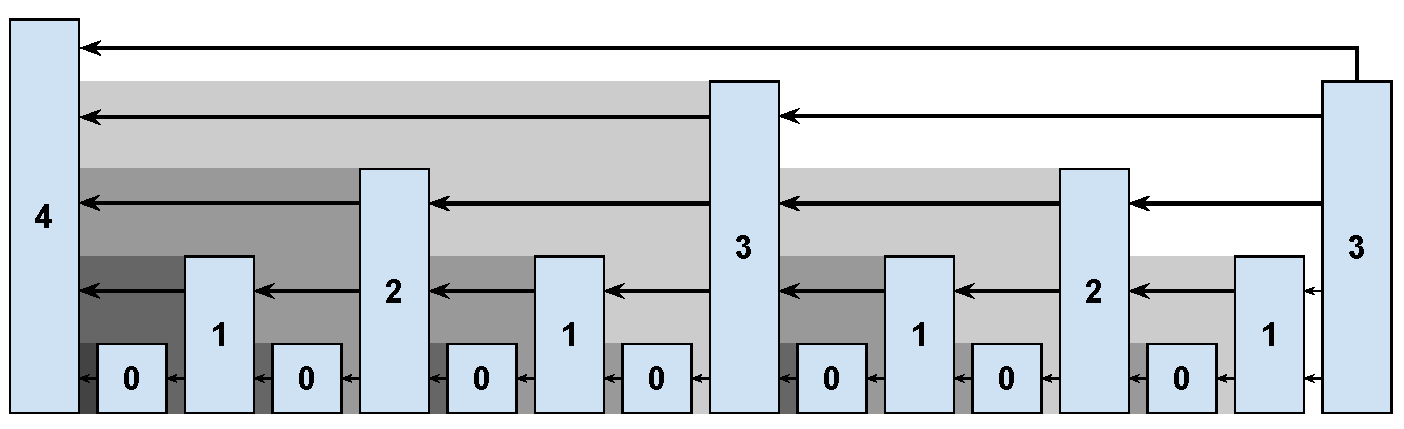
\includegraphics[width=0.9\columnwidth,keepaspectratio]{figures/prelims/level-shadows.pdf}
    \caption{The interlinked blockchain. Each superblock is drawn taller
    according to its achieved level. Each block links to all the blocks that are
    not being overshadowed by their descendants. The most recent (right-most)
    block links to the four blocks it has direct line-of-sight to.}
    \label{fig.hierarchy}
\end{figure}

The exact NIPoPoW protocol works like this: The prover holds a full chain
$\chain$. When the verifier requests a proof, the prover sends the last $k$
blocks of their chain, the suffix $\chi = \chain[-k{:}]$, in full. From the
larger prefix $\chain[{:}-k]$, the prover constructs a proof $\pi$ by selecting
certain superblocks as representative samples of the proof-of-work that took
place. The blocks are picked as follows. The prover selects the \emph{highest}
level $\mu^*$ that has at least $m$ blocks in it and includes all these blocks
in their proof (if no such level exists, the chain is small and can be sent in
full). The prover then iterates from level $\mu = \mu^* - 1$ down to $0$. For
every level $\mu$, it includes sufficient $\mu$-superblocks to cover the last
$m$ blocks of level $\mu + 1$, as illustrated in
Algorithm~\ref{alg.nipopow-prover}. Because the density of blocks doubles as
levels are descended, the proof will contain in expectation $2m$ blocks for each
level below $\mu^*$. As such, the total proof size $\pi \chi$ will be
$\Theta(m\log|\chain| + k)$. Such proofs that are polylogarithmic in the chain
size constitute an exponential improvement over traditional SPV clients and are
called \emph{succinct}.

\noindent \textbf{Verifier.} Upon receiving two proofs $\pi_1\chi_1,
\pi_2\chi_2$ of this form, the NIPoPoW verifier first checks that $\lvert
\chi_1 \rvert = \lvert \chi_2 \rvert = k$ and that $\pi_1 \chi_1$ and $\pi_2
\chi_2$ form valid chains. To check that they are valid chains, the verifier
ensures every block in the proof contains a pointer to its previous block
inside the proof through either the \emph{previd} pointer in the block header,
or in the interlink vector. If any of these checks fail, the proof is rejected.
It then compares $\pi_1$ against $\pi_2$ using the $\leq_m$ operator, which
works as follows. It finds the lowest common ancestor block $b = (\pi_1 \cap
\pi_2)[-1]$; that is, $b$ is the most recent block shared among the two proofs.
Subsequently, it chooses the level $\mu_1$ for $\pi_1$ such that $\lvert
\pi_1\{b{:}\}\upchain^{\mu_1} \rvert \geq m$ (i.e., $\pi_1$ has at least $m$
superblocks of level $\mu_1$ following block $b$) and the value $2^{\mu_1}
\lvert \pi_1\{b{:}\}\upchain^{\mu_1} \rvert$ is maximized.  It chooses a level
$\mu_2$ for $\pi_2$ in the same fashion. The two proofs are compared by
checking whether $2^{\mu_1} \lvert \pi_1\{b{:}\}\upchain^{\mu_1} \rvert \geq
2^{\mu_2} \lvert \pi_2\{b{:}\}\upchain^{\mu_2} \rvert$ and the proof with the
largest score is deemed the winner. The comparison is illustrated in
Algorithm~\ref{alg.nipopow-verifier}.

\begin{algorithm}[H]
    \caption{\label{alg.nipopow-verifier}The \textsf{Verify} algorithm
    for the NIPoPoW protocol}
    \begin{algorithmic}[1]
        \Function{{\sf best-arg}$_m$}{$\pi, b$}
            \Let{M}{\{\mu: |\pi\upchain^\mu\{b:\}| \geq m\} \cup \{0\}}
            \Comment{Valid levels}
            \State\Return{$\max_{\mu \in M}\{2^\mu  \cdot |\pi\upchain^\mu\{b:\}|\}$}
            \Comment{Score for level}
        \EndFunction
        \Operator{$\pi_A \geq_m \pi_B$}
            \Let{b}{(\pi_A \cap \pi_B)[-1]}
              \Comment LCA
            \State\Return{$\textsf{best-arg}_m(\pi_A, b) \geq
                           \textsf{best-arg}_m(\pi_B, b)$}
        \EndOperator
        \Function{\sf Verify$^Q_{m,k}$}{$\mathcal{P}$}
            \Let{\tilde\pi}{(\text{Gen})}
              \Comment{Trivial anchored blockchain}
            \For{$(\pi, \chi) \in \mathcal{P}$}
                \Comment{Examine each proof in $\mathcal{P}$}
                \If{$\mathsf{validChain}(\pi \chi)
                    \land |\chi| = k
                    \land \pi \geq_m \tilde\pi$}
                    \State{$\tilde\pi \gets \pi$}
                    \State{$\tilde\chi \gets \chi$}
                    \Comment{Update current best}
                \EndIf
            \EndFor
            \State\Return{$\tilde{Q}(\tilde\chi)$}
        \EndFunction
    \vskip8pt
    \end{algorithmic}
\end{algorithm}


In the case of the infix proofs there are some additional things that need to
be considered. An adversary prover could skip the blocks of interest and
present an honest and longer chain that, if only the suffix verifier where to
be used, is considered a better proof. For that reason, the last step of the
algorithm in the suffix verifier is changed to not only store the best proof
but also combine the two proofs by including all of the ancestor blocks of the
losing proof. This is guaranteed to include the blocks of interest. The
resulting best proof is stored as a DAG(Directed Acyclic Graph), as in
Algorithm~\ref{alg.nipopow-verifier-infix}

\begin{algorithm}
    \caption{\label{alg.nipopow-verifier-infix}The \textsf{verify} algorithm
    for the NIPoPoW infix protocol}
    \begin{algorithmic}[1]
        \Function{\sf ancestors}{$B, \textsf{blockById}$}
            \If{$B = \text{Gen}$}
                \State\Return{$\{B\}$}
            \EndIf
            \Let{\chain}{\emptyset}
            \For{$\textsf{id} \in B.\textsf{interlink}$}
                \If{$\textsf{id} \in \textsf{blockById}$}
                    \Let{B'}{\textsf{blockById}[\textsf{id}]}
                    \Comment{Collect into DAG}
                    \Let{\chain}{\chain \cup \textsf{ancestors}(B', \textsf{blockById})}
                \EndIf
            \EndFor
            \State\Return{$\chain \cup \{B\}$}
        \EndFunction
        \Function{\sf verify-infx$^D_{\ell,m,k}$}{$\mathcal{P}$}
            \Let{\textsf{blockById}}{\emptyset}
            \For{$(\pi, \chi) \in \mathcal{P}$}
                \For{$B \in \pi$}
                    \Let{\textsf{blockById}[\textsf{id}(B)]}{B}
                \EndFor
            \EndFor
            \Let{\tilde\pi}{\text{best }\pi\in\mathcal{P}\text{ according to suffix verifier}}
            \State\Return{$D(\textsf{ancestors}(\tilde\pi[-1],
            \textsf{blockById}))$}
        \EndFunction
    \vskip8pt
    \end{algorithmic}
\end{algorithm}


\noindent
\textbf{Hard Forks.}
Blockchain protocols can be upgraded using hard or soft
forks~\cite{buterinforks}. In a \emph{hard fork}, blocks produced by
upgraded miners are not accepted by unupgraded miners. It is simplest to
introduce interlinks using a hard fork by mandating that interlink pointers are
included in additional fields in the block header. Unupgraded miners will not
recognize these fields and will be unable to parse upgraded blocks.
To ensure the block header is of constant size, instead of including all these
superblock pointers in the block header individually, they are organized into a
Merkle Tree of interlink pointers and only the root of the Merkle Tree is
included in the block header. In this case, the NIPoPoW prover that wishes to
show a block $b$ in their proof is connected to its more recently preceding
$\mu$-superblock $b'$, also includes a Merkle Tree proof proving that $H(b')$ is
a leaf in the interlink Merkle Tree root included in the block header of $b$.
The verifier has the additional job of verifying the veracity of these Merkle
inclusion proofs.

\noindent
\textbf{Soft Forks.}
In \emph{soft forks}, blocks created by unupgraded miners are not accepted by
upgraded miners, but blocks created by upgraded miners are accepted by
unupgraded miners. As such, any additional data introduced by the upgrade must
be included in a field that is treated like a comment by an unupgraded miner.
To interlink the chain via a soft fork, the interlink Merkle Tree root is
placed in the \emph{coinbase} transaction instead of the block header. Upgraded
miners include the correct interlink Merkle Tree root in their coinbase.
Upgraded miners receiving a new block validate that the interlink Merkle Tree
root is correct before accepting a block as valid. As this root can be
calculated in a deterministic manner from the previous blocks in the chain, it
can easily be validated. Unupgraded miners ignore this data and accept the block
regardless of whether it exists. The success of the fork depends on the majority
of the miner population upgrading. Whenever the NIPoPoW prover wishes to show that a
block $b$ in the proof contains a pointer to its most recently preceding
$\mu$-superblock $b'$, it must then accompany the block header of $b = s \conc
\overline{x} \conc ctr$ with the coinbase transaction $\coinbase$ of $b$ as well
as two Merkle Tree proofs: One proving that the coinbase transaction $\coinbase$
is in $\overline{x}$, and one proving that $H(b')$ is a leaf in the interlink
Merkle Tree whose root is included in $\coinbase$.

% \section{The Hash-and-Resubmit Pattern}

We now introduce a novel design pattern for Solidity smart contracts that
results into massive gas optimization due to the elimination of expensive
storage operations.

\textbf{Motivation.}
% This part is maybe too shallow. Consider deleting it. >>>> In the Ethereum
% blockchain, Turing-complete smart contracts were introduced. In order to
% prevent accidental or adversarial DoS phenomena such as infinite loops of
% code, contract invocations are bounded by an amount of gas units~\cite{wood,
% buterin}.  <<<<
It is essential for smart contracts to store data in the blockchain. However,
interacting with the storage of a contract is among the most expensive
operations of the EVM~\cite{wood, buterin}. Therefore, only necessary data
should be stored and redundancy should be avoided when possible. This is
contrary to conventional software architecture, where storage is considered
cheap. Usually, the performance of data access in traditional systems is
related with time. In Ethereum, however, performance is related to gas
consumption. Access to persistent data costs a substantial amount of gas, which
has a direct monetary value. One way to mitigate gas cost of reading variables
from the blockchain is to declare them public.  This leads to the creation of a
\emph{getter} function in the background, allowing free access to the value of
the variable. But this treatment does not prevent the initial population of
storage data, which is significantly expensive for large size of data.
Towards the goal of implementing gas-efficient smart contracts, several
patterns have been proposed~\cite{contract-opt-1, contract-opt-2,
contract-opt-3, contract-opt-4}.

By using the \emph{hash-and-resubmit} pattern, large structures are omitted
from storage entirety, and are contained in memory. When a function call is
performed, the signature and arguments of the function is included in the
transactions field of the body of a block. The contents of blocks are public to
the network, therefore this information is locally available to full nodes. By
simply observing blocks, a node retrieves data sent to the contract by other
users. To interact publicly with this data without the utilization storage, the
node \emph{resends} the observed data to the blockchain. The concept of
resending data is redundant in conventional systems. However, this technique
is very efficient to use in Solidity due to the significantly lower gas cost
of memory operations in relation with storage operations.

\begin{figure*}[h]
    \begin{center} 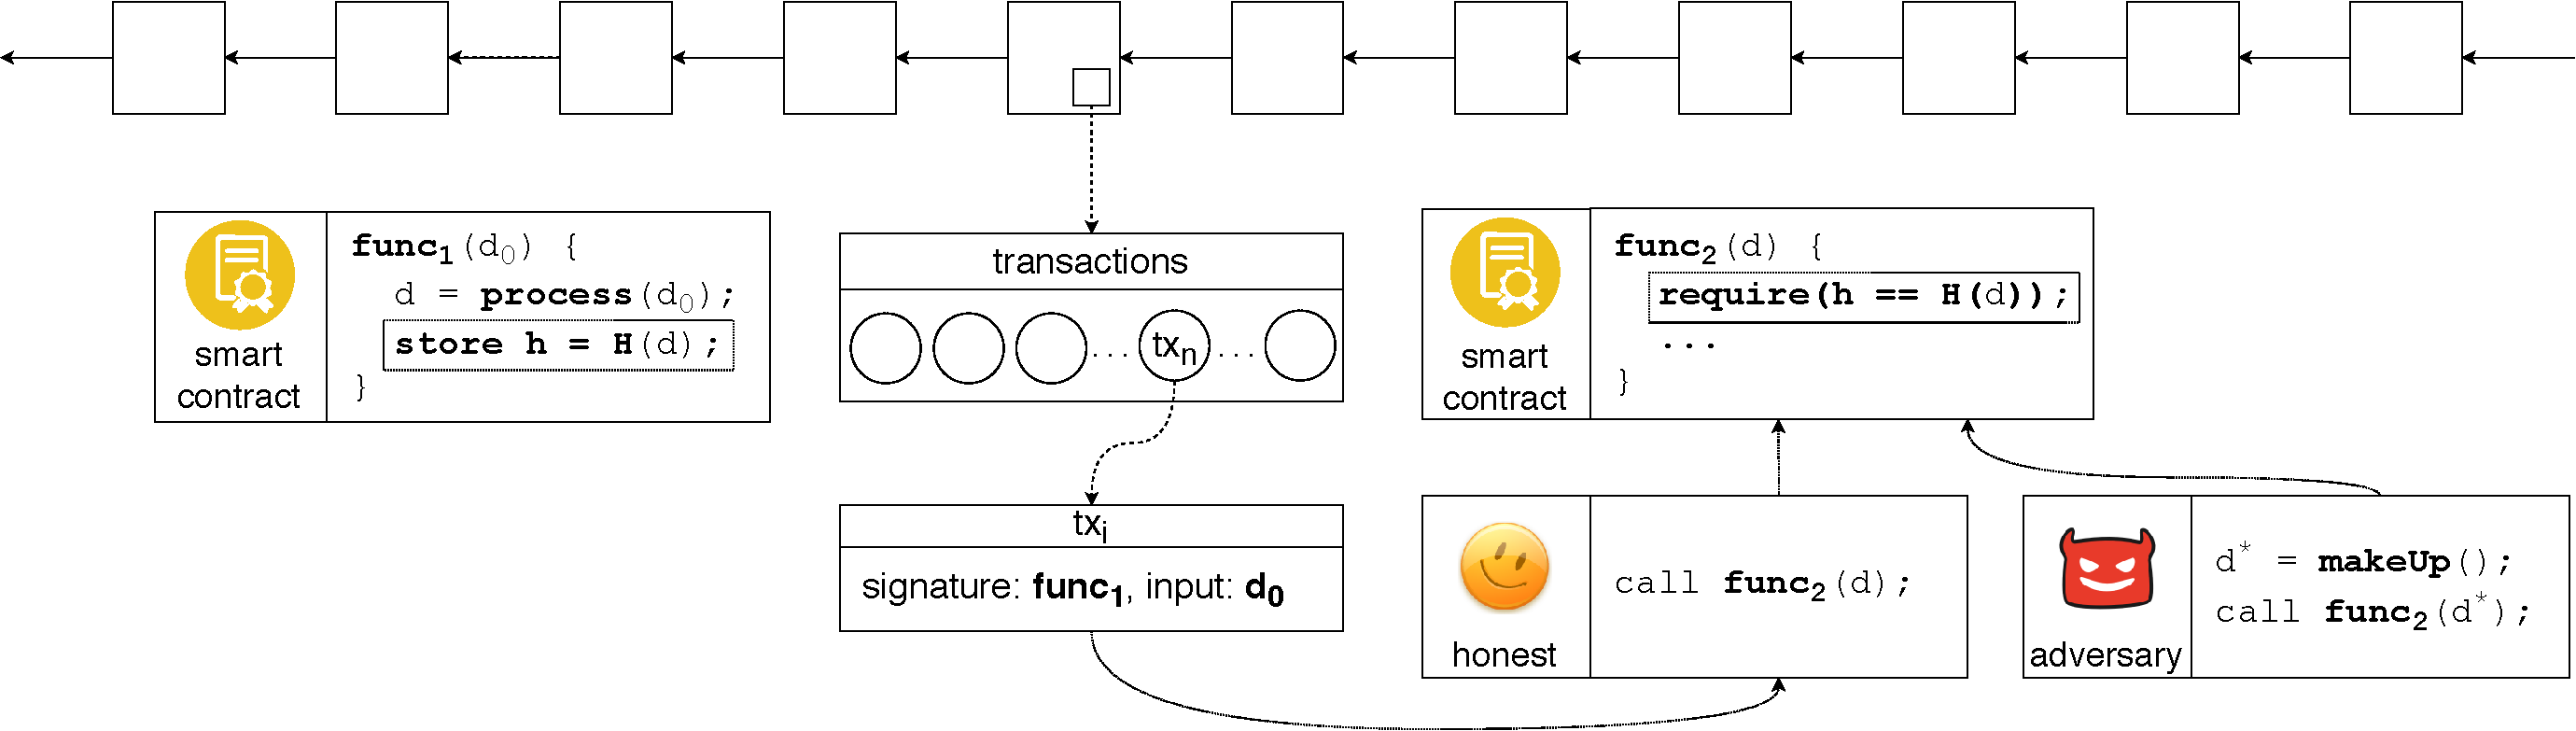
\includegraphics[width=1\textwidth]{figures/har-pattern.pdf}
    \end{center}

    \caption{The \emph{hash-and-resubmit} pattern. In Stage 1, an invoker calls
        \proc$_1$($\data_0$). $\data_0$ is processed on-chain and $\data$ is
        generated. The signature of $\data$ is stored in the blockchain as the
        digest of a hash function \textsf{H}(). In Stage 2, a full node that
        observes invocations of $\proc_1$ retrieves $\data_0$, and generates
        $\data$ by performing the analogous processing on $\data_0$
        \emph{off-chain}. An adversarial observer potentially alters $\data$.
        Finally, in Stage 3, the observer invokes $\proc_2$($\data^*$). In
        $\proc_2$, the validation of $\data$ is performed, reverting the
        function call if the signatures of originally submitted $\data$ does
        not match the signature of $\data^*$. By applying the
        \emph{hash-and-resubmit pattern}, only fixed-size signatures of data
        need to be maintained on the blockchain replacing arbitrarily large
        structures.}

        \label{fig:har-pattern}
\end{figure*}

\noindent
\textbf{Applicability.}
We now list the cases in which the \emph{hash-and-resubmit} pattern is
efficient to use:

The situations in which the \emph{hash-and-resubmit} pattern can be applied are
the following:
\begin{enumerate}
    \item The application is a Solidity smart contract.
    \item Read/write operations are performed in large arrays that exist in
        storage. Rehashing variables of small size may result to negligible
        gain or even performance loss.
    \item The entity that operates on the structures is a full node and
        observes function calls to the smart contract.
\end{enumerate}

\noindent \textbf{Participants and collaborators.} The first participant is the
smart contract $\contract$ that accepts function calls. Another participant is
the invoker $\invoker$, who dispatches a large array $\data_0$ to $\contract$
via a function \texttt{\proc$_1$}($\data_0$). Note that $\data_0$ is
potentially processed in $\proc_1$, resulting to $\data$. The last participant
is the observer $\observer$, who is a full node that observes transactions
towards $\contract$ in the blockchain. This is possible because nodes maintain
the blockchain locally. After observation, $\observer$ retrieves data $\data$.
Since this is an off-chain operation, a malicious $\observer$ potentially
alters $\data$ before interacting with $\contract$. We denote the
potentially modified $\data$ as $\datas$. Finally, $\observer$ acts as an
invoker by making a new call to $\contract$, \texttt{\proc$_2$}($\datas$). The
verification that $\data = \datas$, which is a prerequisite for the secure
functionality of the underlying contract consists a part of the pattern and is
performed in \texttt{\proc$_2$}.

\noindent \textbf{Implementation.} The implementation of this pattern is
divided in two parts. The first part covers how $\datas$ is retrieved by
$\observer$, whereas in the second part the verification of $\data=\datas$ is
realized. The challenge here is twofold:

\begin{enumerate}

    \item Availability: $\observer$ must be able to retrieve $\data$ without
        the need of accessing on-chain data.

    \item Consistency: $\observer$ must be prevented from dispatching $\datas$
        that differs from the originally submitted $\data$.

\end{enumerate}

\noindent
\emph{Hash-and-resubmit} technique is performed in two
stages to face these challenges: (a) the \emph{hash} phase, which addresses
\emph{consistency}, and (b) the \emph{resubmit} phase which addresses
\emph{availability} and \emph{consistency}.

\noindent \textsf{Addressing availability:} During \emph{hash} phase,
$\invoker$ makes the function call \texttt{\proc}$_1$($\data_0$). This
transaction, which includes a function signature (\texttt{\proc$_1$}) and the
corresponding data ($\data_0$), is added in a block by a miner. Due to
blockchain's transparency, the observer of \texttt{\proc}$_1$, $\observer$,
retrieves a copy of $\data_0$, without the need of accessing contract data. In
turn, $\observer$ performs \emph{locally} the same set of on-chain instructions
operated on $\data_0$ generating $\data$. Thus, availability is addressed
through observability.

\noindent \textsf{Addressing consistency} We prevent an adversary $\observer$
from altering $\datas$ by storing the \emph{signature} of $\data$ in contract's
state during the execution of \texttt{\proc$_1$($\data$)} by $\invoker$. In the
context of Solidity, a signature of a structure is the digest of the
structure's \emph{hash}. The pre-compiled \texttt{sha256} is convenient to use
in Solidity, however we can make use of any cryptographic hash function
\textsf{H()}: \[\textsf{hash} \gets \textsf{H}(\textsf{d})\] Then, in
\emph{rehash} phase, the verification is performed by comparing the stored
digest of $\data$ with the digest of $\datas$.
\[\textsf{require}(\textsf{hash} = \texttt{H}(\datas))\] \noindent In Solidity,
the size of digests is 32 bytes. To persist such a small value in contract's
memory only adds a constant, negligible cost overhead.

We illustrate the application of the \emph{hash-and-resubmit} pattern in
Figure~\ref{fig:har-pattern}.

\noindent \textbf{Sample.} We now demonstrate the usage of the
hash-and-resubmit pattern with a simplistic example. We create a smart contract
that orchestrates a game between two players, $\pla$ and $\plb$. The winner is
the player with the most valuable array. The interaction between players
through the smart contract is realized in two phases: (a) the submit phase and
(b) the contest phase.

\noindent \textsf{Submit phase:} $\pla$ submits an N-sized array, $\arra$ and
becomes the $\holder$ of the contract.

\noindent \textsf{Contest phase:} $\plb$ submits $\arrb$. If
\textsf{compare}($\arrb$, $\arra$) is true, then the $\holder$ of the contract
changes to $\plb$. We provide a simple implementation for \textsf{compare()},
but we can consider any notion of comparison, since the pattern is abstracted
from such implementation details.

We make use of the \emph{hash-and-resubmit} pattern by prompting $\plb$ to
provide \emph{two} arrays to the contract during contest phase: (a) $\arras$,
which is the originally submitted array by $\pla$, possibly modified by $\plb$,
and (b) $\arrb$, which is the contesting array.

We provide two implementations of the above described game.
In Algorithm~\ref{alg:game-storage} we display the storage implementation,
while in Algorithm~\ref{alg:game-memory} we show the implementation
embedding the \emph{hash-and-resubmit} pattern.

\begin{algorithm}
    \caption{\label{alg:game-storage}\textsf{best array} using storage}
    \begin{algorithmic}[1]

    \Contract{best-array}
        \State{$\textsf{best} \gets \emptyset$;
               $\textsf{holder} \gets \emptyset$}
        \Function{\sf submit}{$a$}
        \State \textsf{best} $\gets a$
            \Comment{array saved in storage}
            \State \textsf{holder $\gets$ msg.sender}
        \EndFunction

        \Function{\sf contest}{$a$}
            \State \textsf{require}(\textsf{compare}($a$))
            \State \textsf{holder} $\gets$ \textsf{msg.sender}
        \EndFunction

        \Function{\sf compare}{$a$}
            \State \textsf{require}($|a|$ $\geq$ $|$\textsf{best}$|$)
            \For{$i$ \textbf{in} $|$\textsf{best}$|$}
            \State \textsf{require}($a[i]$ $\geq$ \textsf{best}[i])
            \EndFor
            \State \Return{true}
        \EndFunction
        \EndContract
        \vskip8pt
    \end{algorithmic}
\end{algorithm}

\begin{algorithm}
    \caption{\label{alg:game-memory}\textsf{best array} using hash-and-resubmit pattern}
    \begin{algorithmic}[1]
        \Contract{best-array}
        \State{$\textsf{hash} \gets \emptyset$;
               $\textsf{holder} \gets \emptyset$}

        \Function{\sf submit}{$\arra$}
        \State $\textsf{hash} \gets \textsf{H}(\arra)$
            \Comment{hash saved in storage}
            \State \textsf{holder} $\gets$ \textsf{msg.sender}
        \EndFunction

    \Function{\sf contest}{$\arra^*$, $\arrb$}
    \State \textsf{require}(\textsf{hash256}($\arra^*$) $=$ $hash$)
        \Comment{validate $\arra^*$}
        \State \textsf{require}(\textsf{compare}($\arra^*$, $\arrb$))
        \State \textsf{holder} $\gets$ \textsf{msg.sender}
    \EndFunction
    \Function{\sf compare}{$\arra^*$, $\arrb$}
        \State \textsf{require}($|\arra^*|$ $\geq$ $|\arrb|$)
        \For{$i$ \textbf{in} $|\arra^*|$}
            \State \textsf{require}($\arra^*[i] \geq \arrb[i]$)
        \EndFor
    \EndFunction
    \State \Return{true}
    \EndContract
    \vskip8pt
    \end{algorithmic}
\end{algorithm}


\noindent \textbf{Gas analysis.} The gas consumption of the two above
implementations is displayed in Figure~\ref{fig:har-example}. By using the
\emph{hash-and-resubmit} pattern, the aggregated gas consumption for
\textsf{submit} and \textsf{contest} is decreased by 95\%. This significantly
affects the efficiency and applicability of the contract. Note that, the
storage implementation exceeds the Ethereum block gas limit\footnote{As of July
2020, the Ethereum block gas limit approximates 10,000,000 gas units} for
arrays of size 500 and above, contrary to the optimized version, which consumes
approximately only $1/10^{th}$ of the block gas limit for arrays of 1000
elements.

\begin{figure}[h!]
\begin{center}
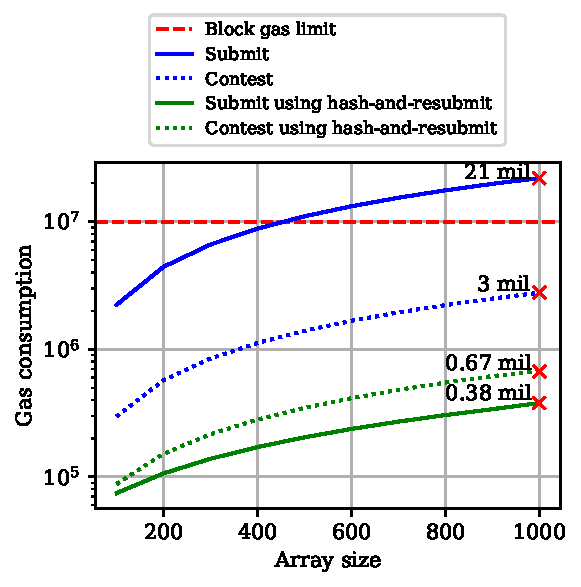
\includegraphics[width=1 \columnwidth]{figures/har-example.pdf}
\end{center}
\caption{Gas-cost reduction using the \emph{hash-and-resubmit} pattern. By
    avoiding gas-heavy storage operations, the aggregated cost of
    \textsf{submit} and \textsf{contest} is decreased significantly by 95\%.}
\label{fig:har-example}
\end{figure}


\noindent \textbf{Variations.}

% Now consider a variation of the above game, in
% which $\pla$ calls \texttt{\proc$_1$(}$\arra$\texttt{)}, and then calls
% \texttt{pickSpan(}$m, n$\texttt{)} that determines the span of $\arra$ which
% can be contested. In reality, $\plb$ only needs to re-send $\arras[m:n]$ in
% order to perform the comparison $\arra[m:n] < \arrb$. However, the digest of
% $\arra$ is calculated by hashing the entire structure. Therefore, the
% $resubmit$ phase cannot be successfully performed by rehashing $\arras[m:n]$,
% because \texttt{H(}$\arra$\texttt{)} $\ne$ \texttt{H(}$\arra[m:n]$\texttt{)}.

In order to enable selective dispatch of a segment of interest, different
hashing schemas can be adopted, such as Merkle Trees (ref) and Merkle Mountain
Ranges (ref). In this variation of the pattern, which we term
\emph{merkle-hash-and-resubmit}, the signature of an array $\textsf{D}$ is
Merkle Tree Root (MTR). In \emph{resubmit} phase, $\textsf{D}[m:n]$ is
dispatched, accompanied by the siblings that reconstruct the MTR of
$\textsf{D}$.

\begin{figure*}[h]
    \begin{center}
        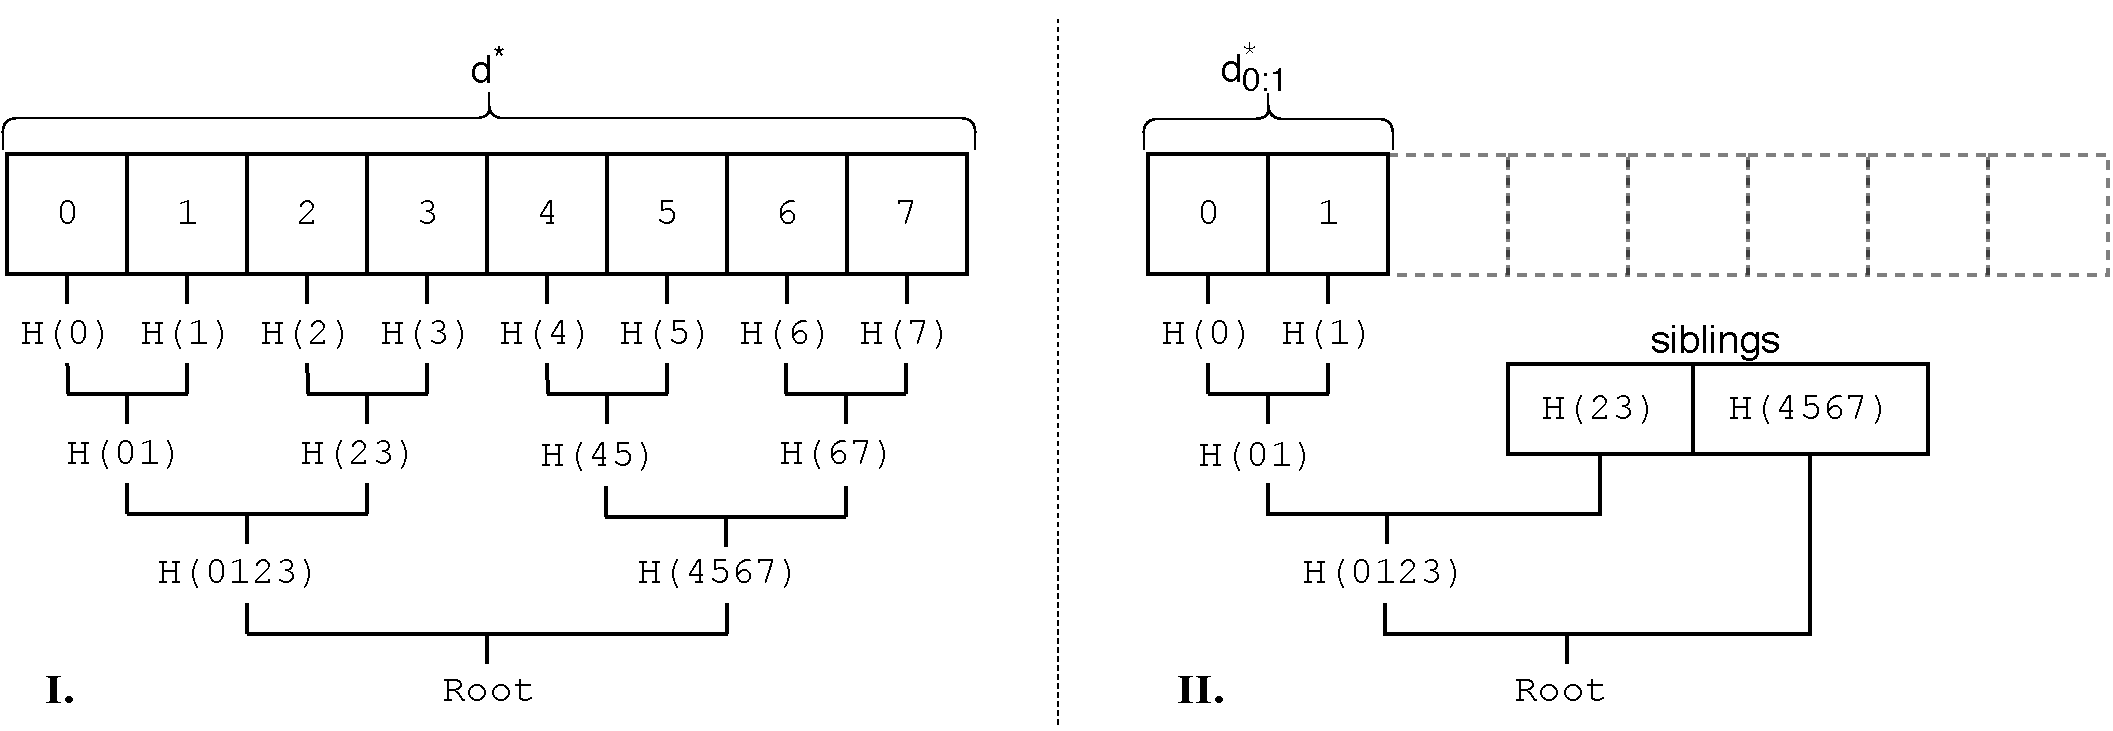
\includegraphics[width=0.8\textwidth]{figures/merkle-har.pdf}
    \end{center}
    \caption{\textbf{I.} The calculation of root in \emph{hash} phase.
    \textbf{II.} The verification of the root in \emph{resubmit} phase.
    \textsf{H}($k$) denotes the digest of element $k$. \textsf{H}($kl$) denotes the
    result of \textsf{H}(\textsf{H}($k$) $|$ \textsf{H}($l$))
}
    \label{fig:merkle-har}
\end{figure*}

This variation of the pattern removes the burden of sending redundant data,
however it implies on-chain construction and validation of the Merkle
construction. In order to construct a MTR for an array $\data$,
$|\data|$ hashes are needed for the leafs of the MT, and $|\data| -
1$ hashes are needed for the intermediate nodes. For the verification, the
segment of interest $\data[m:n]$ and the siblings of the MT are hashed.
The size of siblings is approximately $log_2(|\data|)$. The process of
constructing and verifying the MTR is displayed in Figure
~\ref{fig:merkle-har}.

In Solidity, different hashing operations vary in cost. An invocation of
\textsf{sha256}($\data$), copies $data$ in memory, and then the
\emph{CALL} instruction is performed by the EVM that calls a pre-compiled
contract. In the current state of the EVM, \emph{CALL} costs 700 gas units, and
the gas paid for every word when expanding memory is 3 gas units~\cite{wood}.
Consequently, the expression $1 \times \textsf{sha256}(\data)$ cost less that
$|\data| \times $\textsf{sha}(1) operations. A different cost policy applies
for \textsf{keccak}~\cite{keccak} hash function, where hashing costs 30 gas
units plus 6 additional gas far each word for input data~\cite{wood}. The usage
of \textsf{keccak} dramatically increases the performance in comparison with
\textsf{sha256}, and performs better than plain rehashing if the product of
on-chain processing is sufficiently larger that the originally dispatched data.
Costs of all related operations are listed in Table~\ref{tab:operations-gas}.

The merkle variation can be potentially improved by dividing $\data$ in larger
chunks than 1 element. We leave this analysis for future work.

\begin{table}[!h]
\begin{tabular}{|c|c|}
\hline
\textbf{Operation} & \textbf{Gas cost} \\ \hline
\textsf{load}($\data$)            & $ \data_{bytes} \times 68 $          \\ \hline
\textsf{sha256}($\data$)          & $\data_{words} \times 3 + 700 $     \\ \hline
\textsf{keccak}($\data$)          & $\data_{words} \times 6 + 30 $      \\ \hline
\end{tabular}
\caption{Gas cost of EVM operations as of June 2020.}
\label{tab:operations-gas}
\vspace*{-5mm}
\end{table}


In Table~\ref{tab:har-vs-mhar} we display the operations needed for hashing and
verifying the underlying data for both variations of the pattern as a function
of data size. In Figure~\ref{fig:har-vs-mhar} we demonstrate the gas
consumption for dispatched data of 10KB, and varying size of on-chain
process product.

\newcommand{\mydata}{\data}

\begin{table}[h]
\begin{tabular}{|c|c|c|}
\hline
\textbf{\begin{tabular}[c]{@{}c@{}}phase per\\variance\end{tabular}} &
\textbf{\begin{tabular}[c]{@{}c@{}}plain hash\\and resubmit\end{tabular}} &
\textbf{\begin{tabular}[c]{@{}c@{}}merkle hash\\ and resubmit\end{tabular}} \\ \hline
\textbf{hash} &
\textsf{H}($\mydata$) &
\begin{tabular}[c]{@{}c@{}}
    \textsf{H}($\mydata_{elem}$) $\times\ |\mydata|$ \\ \textsf{H}(digest)
$\times\ (|\mydata|-1)$

\end{tabular} \\ \hline
\textbf{resubmit} &
\textsf{load}($\mydata$) + \textsf{H}($\mydata$) &
\begin{tabular}[c]{@{}c@{}}
    \textsf{load}($\mydata[m{:}n])$ + \\
    \textsf{load}($siblings$) + \\
    \textsf{H}($\mydata[m{:}n])$ + \\
    \textsf{H}($digest$)$\times |siblings|$
\end{tabular} \\ \hline
\end{tabular}

\caption{Summary of operations for \emph{hash-and-resubmit} pattern variations.
$\mydata$ is the product of on-chain operations and $\mydata_{elem}$ is an
element of $\mydata$. \textsf{H} is a hash function, such as \textsf{sha256}
or \textsf{keccak}, $digest$ is the product of \textsf{H}(.) and $siblings$ are
the siblings of the Merkle Tree constructed for $\mydata$.
}

\label{tab:har-vs-mhar}
\vspace*{-10mm}
\end{table}


\begin{figure}[h]
    \begin{center}
        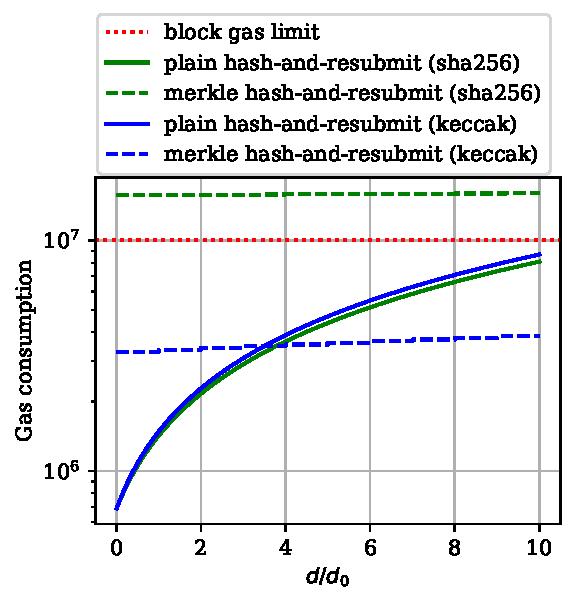
\includegraphics[width=1\columnwidth]{figures/har-vs-mhar.pdf}
    \end{center}
    \caption{Trade-offs between \emph{hash-and-resubmit} variations. In the
    vertical axis the gas consumption is displayed, and in vertical axis the
    size of $\data$ as a function of $\data_0$. The size of $d_0$ is 10KB
    bytes, and the hash function we used is pre-compiled \texttt{sha256}.}
    \label{fig:har-vs-mhar}
\end{figure}

\noindent \textbf{Consequences.} The most obvious consequence of applying the
\emph{hash-and-resubmit} pattern variations is the circumvention of storage
structures, a benefit that saves a substantial amount of gas, especially in the
cases where these structures are large. To that extend, smart contracts that
exceed the Ethereum block gas limit become practical. Furthermore, the pattern
enables off-chain transactions, significantly improving the performance of
smart contracts.

\noindent \textbf{Known uses.} To our knowledge, we are the first to combine
the notion of the transparency of the blockchain with data structures
signatures to eliminate storage variables from Solidity smart contracts by
resubmitting data.

\noindent \textbf{Enabling NIPoPoWs.} We now present how the
\emph{hash-and-resubmit} pattern can used in the context of the NIPoPoW
superlight client. Similar to the aforementioned example, the NIPoPoW verifier
adheres to a submit-and-contest-phase schema, and the inputs of the functions
are arrays that are processed on-chain.

In \emph{submit} phase, a \emph{proof} is submitted, which can be contested by
another user in \emph{contest} phase. The user that initiates the contest,
monitors the traffic of the smart contract~\cite{nipopows}. The input of
\textsf{submit} function includes the submit proof ($\pis$) that indicates the
occurrence of an \emph{event} ($e$) in the source chain, and the input of
\textsf{contest} function includes the contesting proof ($\pic$). A successful
contest of $\pis$ is realized when $\pic$ has a better score. The score
evaluation process is irrelevant to the pattern and remains unchained. The size
of proofs is dictated by the value $m$. We consider $m$ = 15 to be sufficiently
secure.

In previous work~\cite{gglou}, NIPoPoW proofs are maintained on-chain,
resulting to extensive storage operations that limit the applicability of the
contract considerably. We make an analysis to examine the benefit of using the
\emph{hash-and-resubmit} pattern. For our analysis, we create a chain similar
to the Bitcoin chain with the addition of the interlink structure in each block
as in~\cite{gglou}. Our chain spans 650,000 blocks, which are slightly more
than Bitcoin's~\footnote{Bitcoin spans 631,056 blocks as on May 2020. Metrics
by https://www.blockchain.com/}. Then we fork two chains that span 100 and 200
additional blocks, respectively. We illustrate our fork in
Figure~\ref{fig:chains}. We create $\pis$ that describes the smaller chain, and
$\pic$ that describes the larger. In this case, a proof is submitted, and then
contested by a better proof. We select this setting as it provides the maximum
code coverage, and it descries the most gas-heavy scenario.

In Algorithm~\ref{alg:har-nipopow} we show how
hash-and-resubmit pattern is embedded into the NIPoPoW client.

\begin{figure}[!h]
    \begin{center}
        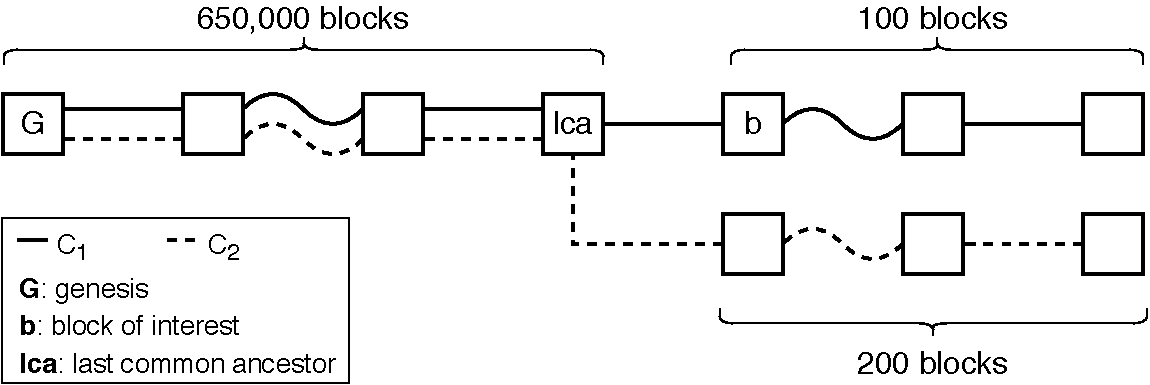
\includegraphics[width=1\columnwidth]{figures/nipopow-subm-cont}
    \end{center}
    \caption{Forked chains for our gas analysis.}
    \label{fig:chains}
\end{figure}

In Figure~\ref{fig:har-nipopow}, we display how results of the
\emph{hash-and-resubmit} implementation differentiate from previous work for
the aggregated cost of \emph{submit} and \emph{contest} phases.  We observe
that by using the \emph{hash-and-resubmit} pattern, we achieve to increase the
performance of the contract 40\%. This is a decisive step towards creating a
practical superlight client.

\newcommand{\genesis}{\textsf{G}}

\begin{algorithm}
    \label{alg:har-nipopow}
    \caption{The \textsf{NIPoPoW} client using hash-and-resubmit pattern}
    \begin{algorithmic}[1]

    \Contract{crosschain}
    \State $\textsf{events} \gets \bot;$ $\genesis \gets \bot$
    \Function{\sf initialize}{$\genesis_{remote}$}
        \State \genesis $\gets \genesis_{remote}$
    \EndFunction
    \Function{\sf submit}{$\pis$, $e$}
        \State \textsf{require}($\pis$[0] = $\genesis$)
        \State \textsf{require}($\textsf{events$[e]$} = \bot$)
        \State \textsf{require}($\textsf{valid-interlink}(\pi)$)
        \State \textsf{DAG} $\gets$ \textsf{DAG} $\cup$ $\pis$
        \State \textsf{events$[e]$.hash} $\gets$ \textsf{H}($\pis$)
        \Comment{enable pattern}
        \State \textsf{ancestors} $\gets$ \textsf{find-ancestors()}
        \State \textsf{events$[e]$.pred} $\gets$
            \textsf{evaluate-predicate}(\textsf{ancestors}, e)
        \State \textsf{ancestors} $=$ $\bot$
    \EndFunction
    \Function{\sf contest}{$\pisa$, $\pic$, $e$}
        \Comment{provide proofs}
        \State \textsf{require}(\textsf{events$[e]$.hash} $=$ \textsf{H}($\pisa$))
        \Comment{verify $\pisa$}
        \State \textsf{require}($\pic$[0] = $\genesis$)
        \State \textsf{require}(\textsf{events}$[e]$ $\ne$ $\bot$)
        \State \textsf{require}(\textsf{valid-interlink}($\pi_{cont}$))
        \State $lca$ = \textsf{find-lca}($\pisa$, $\pic$)
        \State \textsf{require}(\textsf{score}($\pic[:lca]$)
            $>$ \textsf{score}($\pisa[:lca]$))
        \State \textsf{DAG} $\gets$ \textsf{DAG} $\cup$ $\pic$
        \State \textsf{ancestors} $\gets$ \textsf{find-ancestors}(\textsf{DAG})
        \State \textsf{events$[e]$.pred} $\gets$
            \textsf{evaluate-predicate}(\textsf{ancestors}, $e$)
        \State \textsf{ancestors} $=$ $\bot$
    \EndFunction
    \EndContract
    \vskip8pt
    \end{algorithmic}
\end{algorithm}



\begin{figure}[!h]
    \begin{center}
        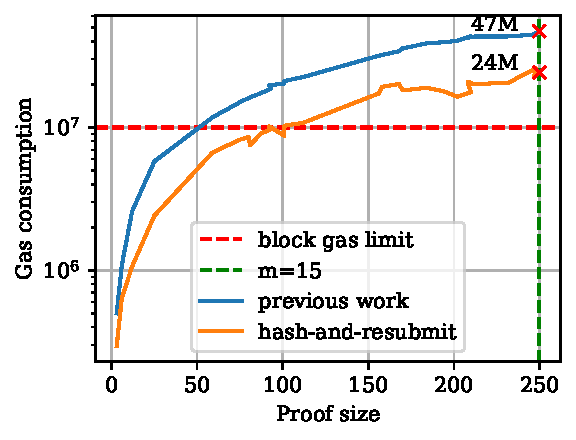
\includegraphics[width=1\columnwidth]{figures/har-nipopows.pdf}
    \end{center}
    \caption{Performance improvement using hash-and-resubmit pattern in
    NIPoPoWs related to previous work for a secure value of $m$. The gas
    consumption decreased by approximately 40\%.}
    \label{fig:har-nipopow}
\end{figure}

% \section{Processing Fewer Blocks}

% \section{Leveraging Multiple Phases}

% \section{Conclusions}


\appendix
% \section{Solidity code}
 % TODO: replace with your brilliant paper!

\bibliographystyle{ACM-Reference-Format}
\bibliography{ccs-sample}

\end{document}
